\documentclass[12pt]{report}
\usepackage{graphicx}
\usepackage{float}
\graphicspath{{resources/}}


\author{Quinn Stevens}
\title{Meetbot}
\date{11/7/17}

\begin{document}
\maketitle
\section*{Executive Summary} \label{execsum}
The following is a report detailing my SDLC coursework project, which I worked on with Shannon Sullivan, Ricard Sol\'e Casas \& Nikhil Kerai. We noticed that nowadays it is quite rare for friendships between employees at a company to extend outside a work capacity. Generally colleagues will socialise with each other at work, or at work-organised activities, but rarely outside of that context. We felt this could be diminishing the social experience of work in modern society.

\vspace{3mm}

\emph{Meetbot} aims to make it easier for work groups, specifically those who use the Slack messaging app for internal communications, to organise out-of-office social gatherings such as lunch or visits to the pub. Users are able to message Meetbot in order to organise gatherings, or to ask if any such gatherings are already being planned and express interest if so.

\vspace{3mm}

Over the course of the project, we designed, built and tested a prototype of \emph{Meetbot} which we were able to present to an audience of Ada College staff and students, along with several external guests, at the end of the 5 days.
\tableofcontents

\chapter{Introduction} \label{intro}
The goal of this project was to use the lean startup methodology, agile and other SDLC concepts covered over the course of the launchpad to design and build a prototype of \emph{Meetbot}, a Slack bot designed to help people organise social meetups.

\vspace{3mm}

Over the course of the 5 day project, all four of us took part in designing the prototype and then later testing it. The programming itself was mainly the work of myself, Shannon and Ricard, and Nikhil made a mockup webpage to be used as a landing page for our product.

\vspace{3mm}

The following report contains an analysis (section \ref{analysis}) describing the problem we were aiming to solve, the technical background of the project and the requirements of the design. This is followed by sections on the design (section \ref{design}) and implementation (section \ref{implementation}) of the prototype, which lay out the major functions of the product and how it is used, and then describe how we created the prototype.

\vspace{3mm}

Finally come testing (section \ref{testing}) and evaluation (section \ref{evaluation}), which lay out how we tested the prototype against our design requirements, and assess how well our finished prototype measures up.

\chapter{Analysis}\label{analysis}
\section{The Problem}
The problem we decided to solve, specifically, was that organising out-of-work activities with colleagues is hard, especially within large or spread-out teams. We thought that making a slackbot to facilitate planning such meetings would be incredibly helpful to our target demographic, whom we defined as "Professionals who would like to organise events outside of work from the comfort of their Slack team".

\vspace{3mm}

For some background, Slack is a popular piece of messaging software which is often used for communication within and between teams in companies, especially those in the tech sector. Slack allows users to set up automated artificial users called bots, which are able to react to messages posted in the chat automatically in order to perform various functions.

\section{Assumptions}\label{assumptions}
We made several assumptions in our initial analysis of the problem. These were the most important of them:

\begin{itemize}
	\item Our slackbot complies with slack's terms of service
	\item People want to socialise outside of work
	\item People use Slack to co-ordinate
	\item People want to see what others are doing and/or be seen
	\item People are familiar with slackbots
	\item People will read detailed help messages
\end{itemize}

We tested these assumptions in various different ways - mainly through a questionnaire and online research - and found the following:\\

\textbf{Our slackbot complies with slack's terms of service}\\
This was the easiest assumption to test - we simply read the Terms \& Conditions of slack. It turned out that what we were doing was indeed sanctioned by the terms, although it looked like it may prove prudent to migrate to a different platform if meetbot started to become popular, as slack reserves the right to rescind API access at any time.

\vspace{3mm}

\textbf{People want to socialise outside of work/People want to see what others are doing}\\
We tested these assumptions by sending out a form through typeform. We distributed this form using viral media techniques, sending it to our friends and asking them to pass it on. In the day or so the form was live, we managed to get almost 70 responses.

\vspace{3mm}

These overwhelmingly supported both of our assumptions. In fact, we were quite surprised that people were so ok with others knowing where they were going.

\vspace{3mm}

\textbf{People use Slack to co-ordinate}\\
In order to test this assumption, we looked at public usage statistics for Slack and two of its closest competitors, Discord and HipChat. It turned out that Slack has much higher usage numbers than Discord, and HipChat don't publish their users at all, which implies that their stats aren't much to look at.

\vspace{3mm}

\textbf{People are familiar with slackbots}\\
We also tested this assumption in our typeform questionnaire, and our results said that most people were indeed familiar with slackbots. However, in later testing it became apparent that although people thought they knew about slackbots, they were not in fact familiar with their usage, so we needed to pivot in order to focus a little more on onboarding.

\vspace{3mm}

\textbf{People will read detailed help messages}\\
We actually didn't test this assumption at all, it was something that became apparent later in the project as we tested and found that people very rarely read the help message that was displayed whenever they tried to type an invalid command. We used this revelation to make plans to make our help message easier to read and parse.

\section{Design Requirements}\label{desreqs}
Looking at the problem and what we wanted our product to allow people to do, we came up with the following design requirements for our bare-bones proof-of-concept prototype.

\begin{itemize}
	\item There must be a help function to enable people to learn more about the bot.
	\item People must be able to create a new event.
	\item People must be able to find out what events are currently being organised.
	\item People must be able to join an event.
\end{itemize}

We also had some further goals which we were unable to achieve within the time available, however we had decided beforehand that these were not needed for a minimum viable product and would be possible to add at a later date. These were:

\begin{itemize}
	\item People should be able to leave an event they have joined.
	\item People should be able to delete an event they created. Also, if all people leave an event, that event should be deleted automatically.
	\item People should be able to set a time for their event, after which it should be automatically deleted.
\end{itemize}


\chapter{Design}\label{design}
\section{Design process}

At the beginning of our design process, we first set out to define the group of people we would be aiming to have as our users. After some discussion we agreed that that group would be "Professionals who would like to organise events outside of work from the comfort of their Slack team". We then set out to define all the assumptions we had made about this group of users, and to test those assumptions to see if we were correct. This we did by creating a user research form with Typeform, and then sending this form out to people we knew in various communities we were a part of. You can see the results of this user research in the analysis section.

\vspace{3mm}

After that we looked at the journeys different user archetypes would take as they used our tool - for instance, the person installing our bot, slack team admins, and just general users on the team. We then broke these down into user stories, and then further into issues we wanted to address. We put these up on a wall on post-it notes as items to complete, and then assigned them to various team members to complete.

\section{Prototype Design}

As a chat bot, \emph{Meetbot} is quite hard to define in terms of a flowchart, so instead we created a bullet point list of things we wanted the bot to be able to do.

\begin{itemize}
	\item \textbf{Help function:} If the user messages the word ``help'' to the bot, the bot should respond with a list of other commands, which will help guide the user in making use of the bot.
	\item \textbf{View function:} If the user says ``What's up?'' to the bot, the bot should respond with a list of the events that are currently being organised, and who is going to each event.
	\item \textbf{Create function:} If the user says ``create'' followed by the name of an event, the bot should create an event under that name.
	\item \textbf{Join function:} If the user types ``join'' followed by a number, the bot should add that user as a participant to the event.
\end{itemize}

\chapter{Implementation}\label{implementation}
\section{Implementation Strategy}
We used the Kanban methodology to organise our work, as we decided that with such a short timeframe in which to implement the project, Scrum would be too unwieldy with its sprints \& standups. Kanban was a lot more flexible, and allowed us to focus our attention on a small number of tasks at a time. We broke down our user stories into features to implement and divided them between ourselves.

\vspace{3mm}

We programmed the bot itself in python, using slack's messaging API and a bot user which we were able to create using their online tools. Python was chosen because it is a very easy language to get something working quickly in, so it is ideal for prototyping. If we were to go on to make a fully fledged product, we might use a different language, but for our purposes Python was perfect. We also used Github for version control and Waffle.io for project management, and we deployed the bot itself as an app on Heroku.

\vspace{3mm}

At first, we delegated tasks between all four of us, with one of us working on each issue. However it quickly became clear that we worked much better when collaborating, so we decided that the programming part of the project should be done in a group. We spent most of the time during the project with myself, Shannon and Ricard programming as a group, using mob programming techniques, and Nik working on designing our landing page, as he had some experience with creating websites and not much with programming, especially not in Python.

\vspace{3mm}

Later on, we switched to working in pairs, with myself and Shannon working on the programming, and Ricard and Nik doing user testing.

\section{Prototype screenshots}
The final bot had functions for providing help, seeing current events, creating events and joining them, as shown here:

\begin{figure}[H]
\caption{If the user sends the message ``help'', \emph{Meetbot} will reply with a list of the various different commands available.}
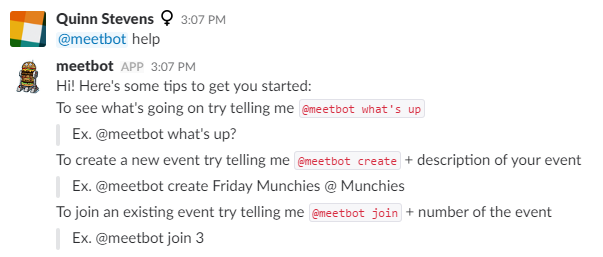
\includegraphics{help}
\end{figure}

\begin{figure}[H]
\caption{The message ``What's up'' will list the currently organised events, along with everyone who's currently going to them.}
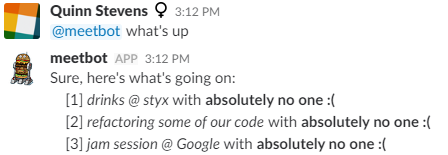
\includegraphics{whatsup}
\end{figure}

\begin{figure}[H]
\caption{If the user types ``Create'' followed by the name of an event, that event will be created by the bot.}
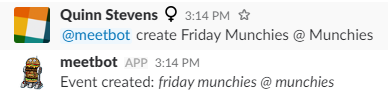
\includegraphics{create}
\end{figure}

\begin{figure}[H]
\caption{Finally, if the user types ``join'' followed by a number, they will be added as a participant to that event.}
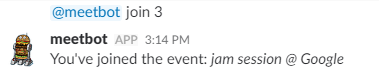
\includegraphics{join}
\end{figure}

\chapter{Testing}\label{testing}
Before we even started implementing the slackbot, we decided it would be useful to know how people would try to use the bot, so we set up a prototype trial. We wrote a script with sample commands and responses, and then Ricard changed his Slack username and profile picture and pretended to be the slackbot. We then went round various people and asked them to try and use the slackbot. This was very useful as it let us know that people as a whole aren't very familiar with how chat bots work. This helped us to reassess some of our assumptions, such as that our users would be 'technically savvy' - we had to redefine what we meant by 'technically savvy' as we hadn't anticipated people having trouble using the bot.

\vspace{3mm}

Later, when we had managed to make a working prototype, Ricard and Nik added the bot to our own slack team and went round various people in the college asking them to try and use the bot. They asked several questions to try and see how users would react to being asked to do certain tasks, and recorded the training sessions so we could use them as data to inform our direction going forward.

\vspace{3mm}

We found that all four of our original design requirements (the help function, and viewing, creating and joining events) had been implemented satisfactorily - users were able to view, create and join events, and to ask the bot for help when they were stuck.

\vspace{3mm}

From the testing we learnt that it was important to keep interaction with the bot as natural-feeling as possible, both by allowing the use of natural-language-like commands ("@meetbot, I'd like to go to Styx for drinks after work" instead of "@meetbot create drinks at Styx after work"), and by making the bot follow a more human-like thought process. There were several features which hadn't occurred to us, but which many of our test users assumed would be possible, for instance the ability to see information about just one event, or only the events they were going to.

\vspace{3mm}

We also discovered the importance of testing \emph{while} building, instead of building something and then testing it. It took us much longer than it should have to learn that our help function was unintuitive - when we tested, many people didn't read it at all, and therefore had no idea of the commands available to them, and for others the wording was ambiguous so they assumed there were commands that weren't listed in the help function, where that was not the case.

\chapter{Evaluation}\label{evaluation}
Overall, this project has been incredibly interesting, and we learnt many things that will hopefully allow us to make better products in the future. We learnt a lot about the value of collaboration and communication between team members, the importance of giving and receiving feedback, and the power of constant iteration and flexible direction in building software.

\vspace{3mm}

Among the things we would like to have done if we had more time were adding more functionality to the actual events, such as the ability to keep track of what time they are happening and who organised them. This would allow things like sending reminders to people before the event, or allowing event organisers to edit or delete events.

\vspace{3mm}

It would also be incredibly important to implement some sort of one-click install feature or an installation wizard, because currently the process of installing the slackbot requires technical knowledge that not everyone will have.

\vspace{3mm}

I now have a much greater understanding of the advantages of the agile approach to software development, as before I had experience working with it, when it was just theory, it seemed to be a lot of effort for not much gain. Now however I see how helpful it is to keeping a project going; and more importantly, keeping it heading in the right direction.
\end{document}
